%%%%%%%%%%%%%%%%%%%%%%%%%%%%%%%%%%%%%%%%%
% Short Sectioned Assignment
% LaTeX Template
% Version 1.0 (5/5/12)
%
% This template has been downloaded from:
% http://www.LaTeXTemplates.com
%
% Original author:
% Frits Wenneker (http://www.howtotex.com)
%
% License:
% CC BY-NC-SA 3.0 (http://creativecommons.org/licenses/by-nc-sa/3.0/)
%
%%%%%%%%%%%%%%%%%%%%%%%%%%%%%%%%%%%%%%%%%

%----------------------------------------------------------------------------------------
%	PACKAGES AND OTHER DOCUMENT CONFIGURATIONS
%----------------------------------------------------------------------------------------
\iffalse
\documentclass[12pt]{ussci} % A4 paper and 11pt font size

\usepackage{graphicx}
\usepackage{caption}
\usepackage{subcaption}
\usepackage{amsmath,amsfonts,amssymb}
\usepackage[version=4]{mhchem}

%better printing of numbers
\usepackage[T1]{fontenc}
\usepackage[english]{babel}
\usepackage{csquotes}
\usepackage{textcomp}
\usepackage{changepage}
\usepackage[titletoc,title]{appendix}

\usepackage{siunitx}
\sisetup{group-separator={,},
     detect-all,
     binary-units,
     list-units = single,
     range-units = single,
     tophrase = --,
     per-mode = symbol-or-fraction,
     separate-uncertainty = true,
     list-final-separator = {, and }
%    scientific-notation = fixed
}
\DeclareSIUnit\atm{atm}

\usepackage{fancyhdr} % Custom headers and footers
\pagestyle{fancyplain} % Makes all pages in the document conform to the custom headers and footers
\fancyhead{} % No page header - if you want one, create it in the same way as the footers below
\fancyfoot[L]{} % Empty left footer
\fancyfoot[C]{} % Empty center footer
\fancyfoot[R]{\thepage} % Page numbering for right footer
\renewcommand{\headrulewidth}{0pt} % Remove header underlines
\renewcommand{\footrulewidth}{0pt} % Remove footer underlines
\setlength{\headheight}{13.6pt} % Customize the height of the header

%\numberwithin{equation}{section} % Number equations within sections (i.e. 1.1, 1.2, 2.1, 2.2 instead of 1, 2, 3, 4)
%\numberwithin{figure}{section} % Number figures within sections (i.e. 1.1, 1.2, 2.1, 2.2 instead of 1, 2, 3, 4)
%\numberwithin{table}{section} % Number tables within sections (i.e. 1.1, 1.2, 2.1, 2.2 instead of 1, 2, 3, 4)

% \setlength\parindent{0pt} % Removes all indentation from paragraphs - comment this line for an assignment with lots of text



%\bibliography{mendeley.bib}
\fi

\documentclass[paper=letter, fontsize=10pt]{scrartcl} % A4 paper and 11pt font size

\usepackage[T1]{fontenc} % Use 8-bit encoding that has 256 glyphs
\usepackage{fourier} % Use the Adobe Utopia font for the document - comment this line to return to the LaTeX default
\usepackage[english]{babel} % English language/hyphenation
\usepackage{amsmath,amsfonts,amsthm} % Math packages
\usepackage{graphicx}
\usepackage{caption}
\usepackage[titletoc,title]{appendix}
%\usepackage{titlesec}
\usepackage{footnote}
\usepackage{changepage}
\usepackage{sectsty} % Allows customizing section commands
\allsectionsfont{\centering \normalfont\scshape} % Make all sections centered, the default font and small caps

\makesavenoteenv{tabular}

\usepackage{fancyhdr} % Custom headers and footers
\pagestyle{fancyplain} % Makes all pages in the document conform to the custom headers and footers
\fancyhead{} % No page header - if you want one, create it in the same way as the footers below
\fancyfoot[L]{} % Empty left footer
\fancyfoot[C]{} % Empty center footer
\fancyfoot[R]{\thepage} % Page numbering for right footer
\renewcommand{\headrulewidth}{0pt} % Remove header underlines
\renewcommand{\footrulewidth}{0pt} % Remove footer underlines
\setlength{\headheight}{13.6pt} % Customize the height of the header



%----------------------------------------------------------------------------------------
%	TITLE SECTION
%----------------------------------------------------------------------------------------

\newcommand{\horrule}[1]{\rule{\linewidth}{#1}} % Create horizontal rule command with 1 argument of height

\title{	
\normalfont \normalsize 
\textsc{ME 552} \\ [25pt] % Your university, school and/or department name(s)
\horrule{0.5pt} \\[0.4cm] % Thin top horizontal rule
\huge Report for Lab 3: Turbulent Flame Speed Measurements \\ % The assignment title
\horrule{2pt} \\[0.5cm] % Thick bottom horizontal rule
}

\author{Andrew Alferman} % Your name

\date{\normalsize\today} % Today's date or a custom date

\begin{document}

\iffalse
%THINGS HERE ARE THE OBJECTIVES TO HIT ON FROM THE LAB 3 FILE
To include in report:

-Respond to questions in the handout

-Conclude by describing what we learned

-Include in appendix documentation about data reduction code and anything else needed to support the discussion

Specifically include:
Process a series of 5 consecutive time-resolved images of the flame for each of the operating conditions and include representative images in the report.  Describe any observed changes for the different conditions and  explain any significance

\fi

\maketitle % Print the title

\section{Introduction}
\label{intro}
A controlled turbulent flame on a burner apparatus was investigated using an intensified charged coupled device (ICCD) camera to study its flow characteristics.  The burner apparatus, which previously had been investigated as part of a flow calibration experiment, produces both a pilot flame and a larger turbulent flame in a variety of Reynolds number and turbulence intensity conditions.  The fuel used in the experiment was methane.  For safety reasons, data for only the smaller pilot flame was obtained in this experiment.  Data from the larger turbulent flame was collected at a separate time, which made it possible for the turbulent flame to be studied by computing the differences between images of the two flames.  Once images of this difference had been obtained, the apparent cross sectional area of the flame was measured.  The objective of this experiment was to familiarize the student with optical measurement devices and techniques, particularly in regard to combustion, and to introduce the student to some of the basic principles regarding combustion physics.


\section{Methodology}
\subsection{Experiment Description}
The turbulent flame was measured in four different configurations by computing the difference in light intensity between the pilot flame and the turbulent flame in each configuration.  Once the difference between the turbulent flames and the pilot flames had been computed, a calibration image was used to calculate the apparent cross sectional area of the flame.  Before the experiment began, the ICCD camera was set up in a fixture at an angle to view the entirety of the flame and the burner apparatus was calibrated in accordance with the procedures detailed in the Laboratory 1 report.  An detailed overview of the calibration of the equipment used in the burner apparatus can also be found in the Laboratory 1 report.  For sake of completeness, the equipment used in Laboratory 1 has been included in Appendix \ref{app:Equip}.  At the onset of the experiment, the ICCD camera was first turned on to allow the equipment to be automatically cooled to its operating temperature, which is cooler than room temperature.  After the camera had fully cooled to its operational temperature, a calibration image was taken.
% ADD IN THE PROCEDURE FOR LAB 1 AS A REFERENCE

The calibration image was taken by placing a ruler directly on top of the burner nozzle and recording one image with the ICCD camera.  The ruler was illuminated with an ultraviolet light source because an ultraviolet lens was affixed to the ICCD camera and the ambient lighting was insufficient to resolve an image in that spectrum.  Once it had been verified that a satisfactory calibration image had been obtained, the ruler was removed and the burner apparatus was started.  After verifying that all equipment was operating normally, the pilot flame was ignited.


After igniting the pilot flame, the test apparatus was allowed to stabilize.  The ICCD camera was then started, taking six pictures every second for one minute, for a total of 360 images that were each saved in one file on the computer.  The images captured the chemiluminescence of the OH* radicals.  After verifying that the file had saved properly, the test apparatus was shut down and the flame was allowed to extinguish.  Finally, the experiment was repeated twice more for a total of 3 separate collections of data to ensure repeatability.


Though it was not witnessed by the students, the experiment was run again using the same procedures as before, however the turbulent flame was started instead of shutting down the experiment.  The turbulent flame was run using two different Reynolds numbers and two different turbulence intensities for a total of four different conditions.  The Reynolds numbers were controlled by increasing the fuel and air flow rate through the burner.  The turbulence intensity was controlled by using a turbulence generator as described by Fillo in \cite{Fillo2015}.  The turbulence generator operated by opening or closing the turbulence generator and thus changing the blockage ratio.


\subsection{Equipment Used}
A list of all of the equipment used can be found in Appendix \ref{app:Equip}.


\subsection{Data Analysis}
After completing all measurements of the flame, the test apparatus was shut down and the data was processed using the MATLAB code included in appendix \ref{app:Code}.  This code processed the images and produced a series of five time-resolved images of the flame for each of the operating conditions.  The code then read the averaged images of the flame, counting the number of pixels which exhibited a light magnitude greater than a given threshold.  Using the calibration image of the ruler, the program calculated the approximate dimensions of every pixel, which allowed the apparent flame area to be calculated as follows:
\begin{equation}
A = P_{flame}l_{calibration}^2
\end{equation}
in which $A$ is the apparent flame cross sectional area, $P_{flame}$ is the number of pixels observed to have a light magnitude greater than the threshold, and $l_{calibration}$ is the calibration length, which was in turn determined using the equation
\begin{equation}
l_{calibration} = \frac{l_{ruler}}{P_{ruler}}
\end{equation}
in which $l_{ruler}$ is a length measured by the ruler in the calibration image, and $P_{ruler}$ is the number of pixels between the two points measured on the ruler.


\section{Assumptions}
The apparent cross sectional area was assumed to be an accurate indication of the flow characteristics of the flame.  This assumption is not technically correct, however it is considered to be sufficient for the purposes of this experiment.  Calculation of values that may be used as accurate metrics of flame characteristics require sophisticated techniques that are beyond the scope of this course.  See \cite{Fillo2017} for additional information.


The apparent cross sectional area of the flame has no exact definition, and therefore assumptions had to be made regarding its nature.  As instructed in class, it was assumed to be defined as the region in which the light intensity exceeds a defined albeit arbitrary magnitude.  This definition lacks the precision of many of the more rigorous terms used in \cite{Fillo2015} for example, however it was determined to be sufficient for the purposes of this exercise.  In the case of this lab report, the magnitude used to define the apparent cross sectional area was 24.  The author is unaware of any physical meaning behind this number, however use of this number yielded a well defined region in the figures of the average plots constructed using the data from the experiment and MATLAB.


In the interests of reducing the time required to complete this laboratory report, an uncertainty analysis was not conducted as part of the current experiment, however a detailed uncertainty analysis has previously been completed by Fillo \cite{Fillo2017}.

\section{Results}
Time-resolved images of the flame for each of the operating conditions have been included in appendix \ref{app:Flames}.  The first image of each figure is an averaged image of all images taken under the stated operating condition.  Because it is averaged over many different images, it is smoother than any single image.  All data regarding the flame size was measured using this averaged image.  The subsequent images are the first and last images taken for the stated test condition.  These images are subject to a large degree of variation due to the turbulent nature of the flame.

The apparent flame cross sectional areas for each of the operating conditions can be found in table \ref{tab:flameareas} below:

\begin{table}[ht]
\begin{adjustwidth}{-1in}{-1in}
\begin{center}
\begin{tabular}{| c | c | c | c|}
 \hline
 Re = 5,000 & Re = 5,000 & Re = 10,000 & Re = 10,000 \\
 Turbulence Intensity: & Turbulence Intensity: & Turbulence Intensity: & Turbulence Intensity: \\
 High & Low & High & Low\\
\hline
 3.29 $\textnormal{cm}^2$ & 3.54 $\textnormal{cm}^2$& 6.81 $\textnormal{cm}^2$ & 7.22 $\textnormal{cm}^2$\\
 \hline
 \end{tabular}
 \caption{Apparent Flame Cross Sectional Area}\label{tab:flameareas}
 \end{center}
 \end{adjustwidth}
\end{table}

As can be seen, the apparent cross sectional area increased greatly by increasing the Reynolds number, and increased slightly by using a low turbulence intensity instead of a high turbulence intensity.  The flame grew when the Reynolds number increased due to the larger mass and volumetric flow rates.  The increased flow rate meant that the burning fuel was carried further as it combusted, effectively stretching out the flame.  At the same time, the higher Reynolds number meant that the flame had greater mixing and interaction with oxygen from the surrounding environment, which facilitated combustion.  Counterintuitively, the increased turbulence intensity caused the flame to occupy less volume.  The reasons for the decrease in volume are complicated, however one potential cause is that the increase in turbulence intensity is associated with a wrinkling of the flame front.  This wrinkling means that the flame would have a greater surface area for the same volume.  The surface area of the flame is proportional to the amount of oxygen that will come into contact with unburnt fuel, therefore the increased surface area causes the turbulent flame speed will increase, which in turn causes the fuel to burn faster.  Because the amount of fuel remains constant in both high turbulence intensity and low turbulence intensity conditions, the faster burning fuel results in a flame with a smaller volume.


\section{Conclusion}
Optical measurements provided an effective means of measuring the size of a flame.  This size measurement can be used to gain insight into the fundamental physics behind combustion mechanisms.  In this experiment it was verified that the size of the flame increased with increasing Reynolds number, and slightly decreased with increasing turbulence intensity.  Although the increase in size due to an increase in Reynolds number was an intuitive result, I learned that an increase in turbulence intensity and the associated increase in turbulent flame speed can actually result in a smaller flame instead of a larger one.  This is an important observation because it provides great insight into the fundamental physics of combustion.


\bibliography{mendeley}
\bibliographystyle{unsrt}


\clearpage
\begin{appendices}
%\setcounter{equation}{0}
%\setcounter{figure}{0}
%\setcounter{table}{0}

\section{Flame Images}\label{app:Flames}

\begin{figure}[ht]
\centering
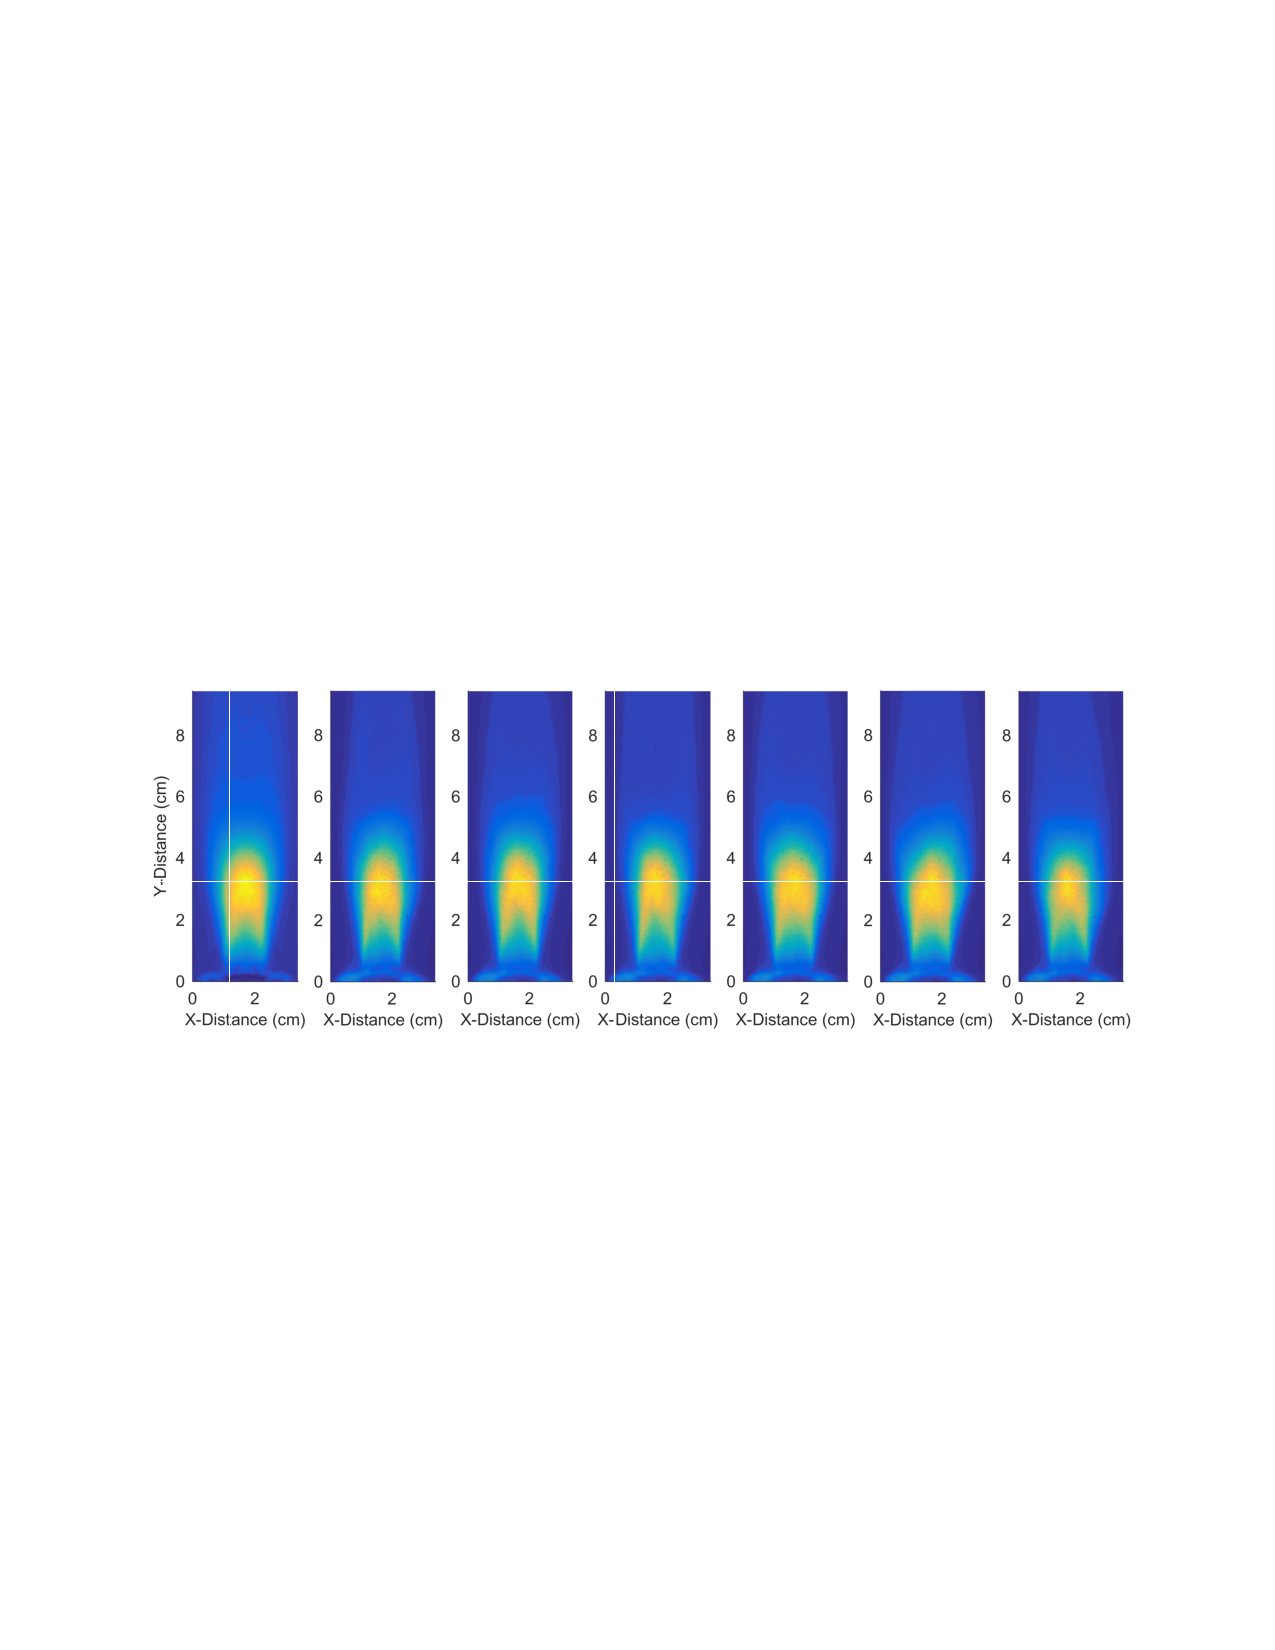
\includegraphics[width=.95\textwidth]{Re5kHigh.pdf}
\caption{Flame with a Reynolds number of 5,000 and high turbulence intensity.  The combined time-averaged flame is shown on the left, and the flame area was found to be approximately 3.29 $\textnormal{cm}^2$}
\label{fig:5high}
\end{figure}

\begin{figure}[ht]
\centering
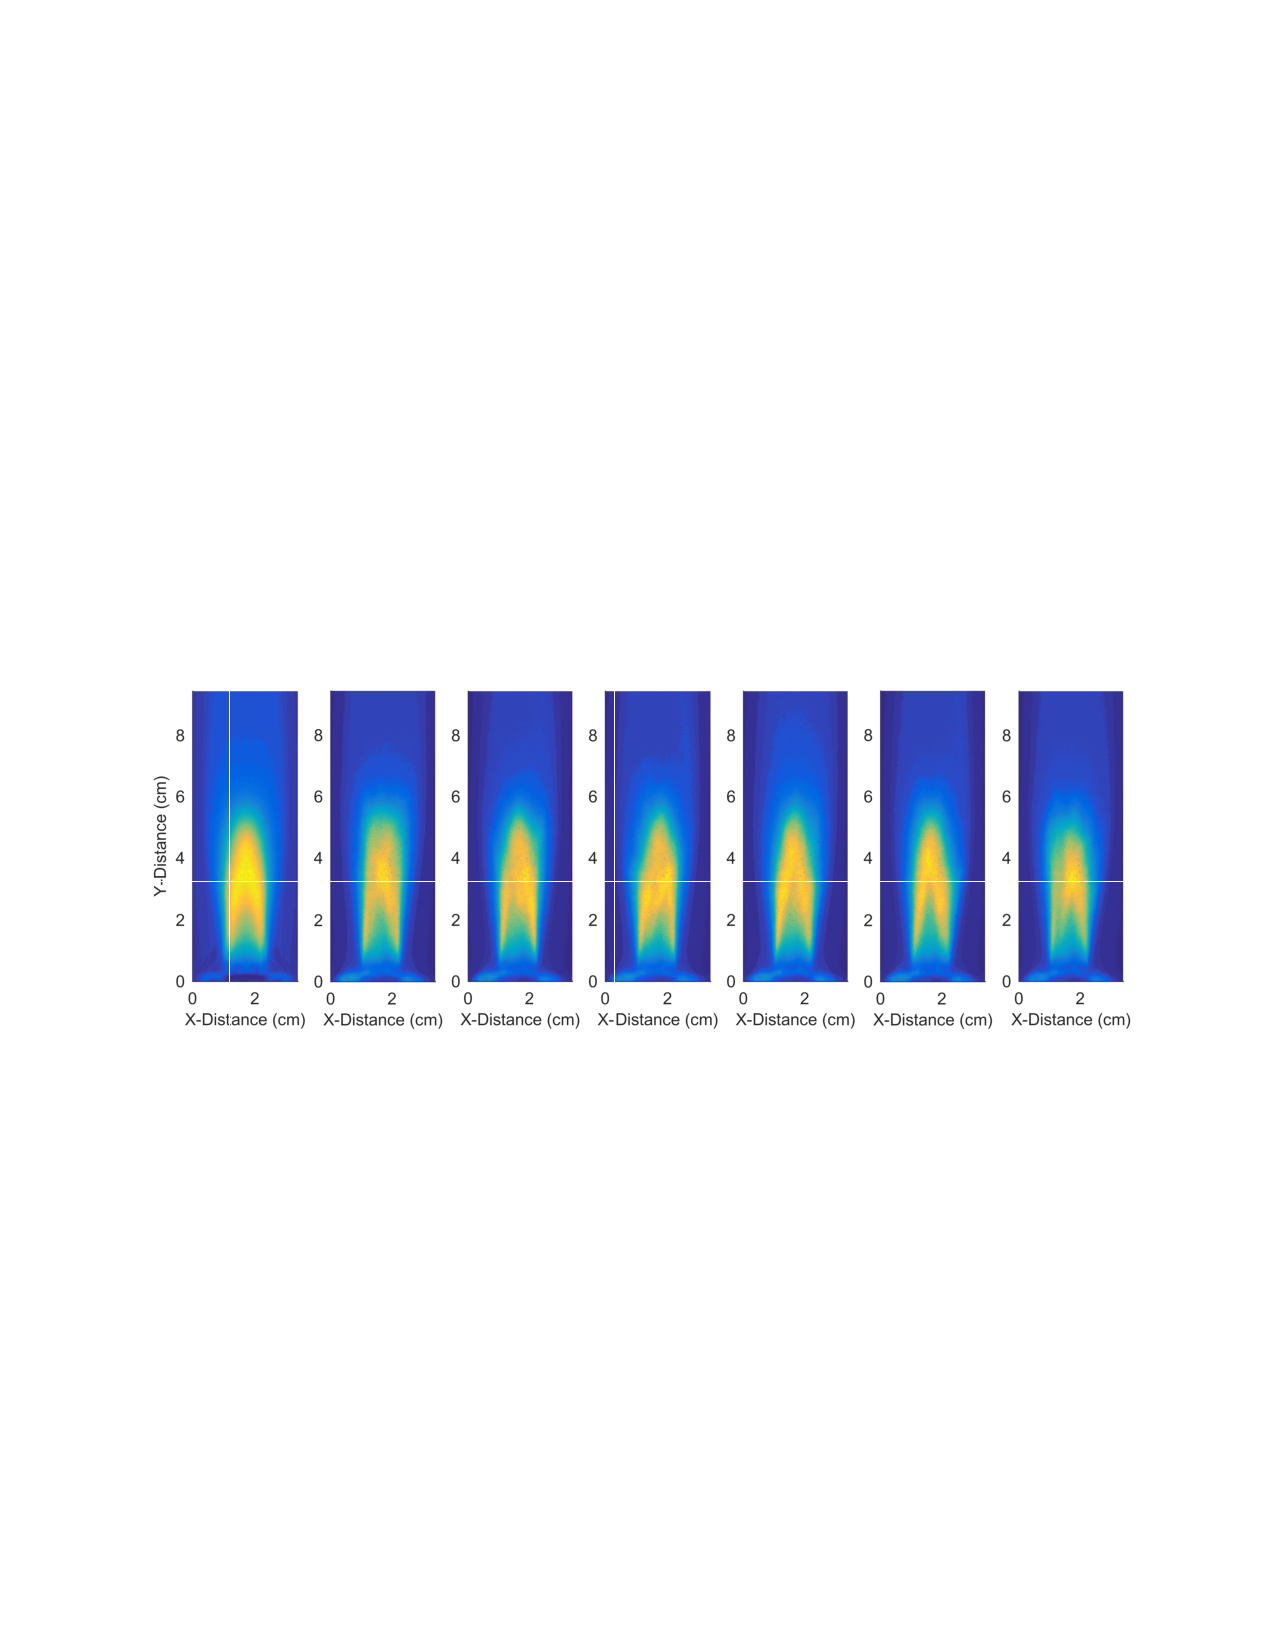
\includegraphics[width=.95\textwidth]{Re5kLow.pdf}
\caption{Flame with a Reynolds number of 5,000 and low turbulence intensity.  The combined time-averaged flame is shown on the left, and the flame area was found to be approximately 3.54 $\textnormal{cm}^2$}
\label{fig:5low}
\end{figure}

\begin{figure}[ht]
\centering
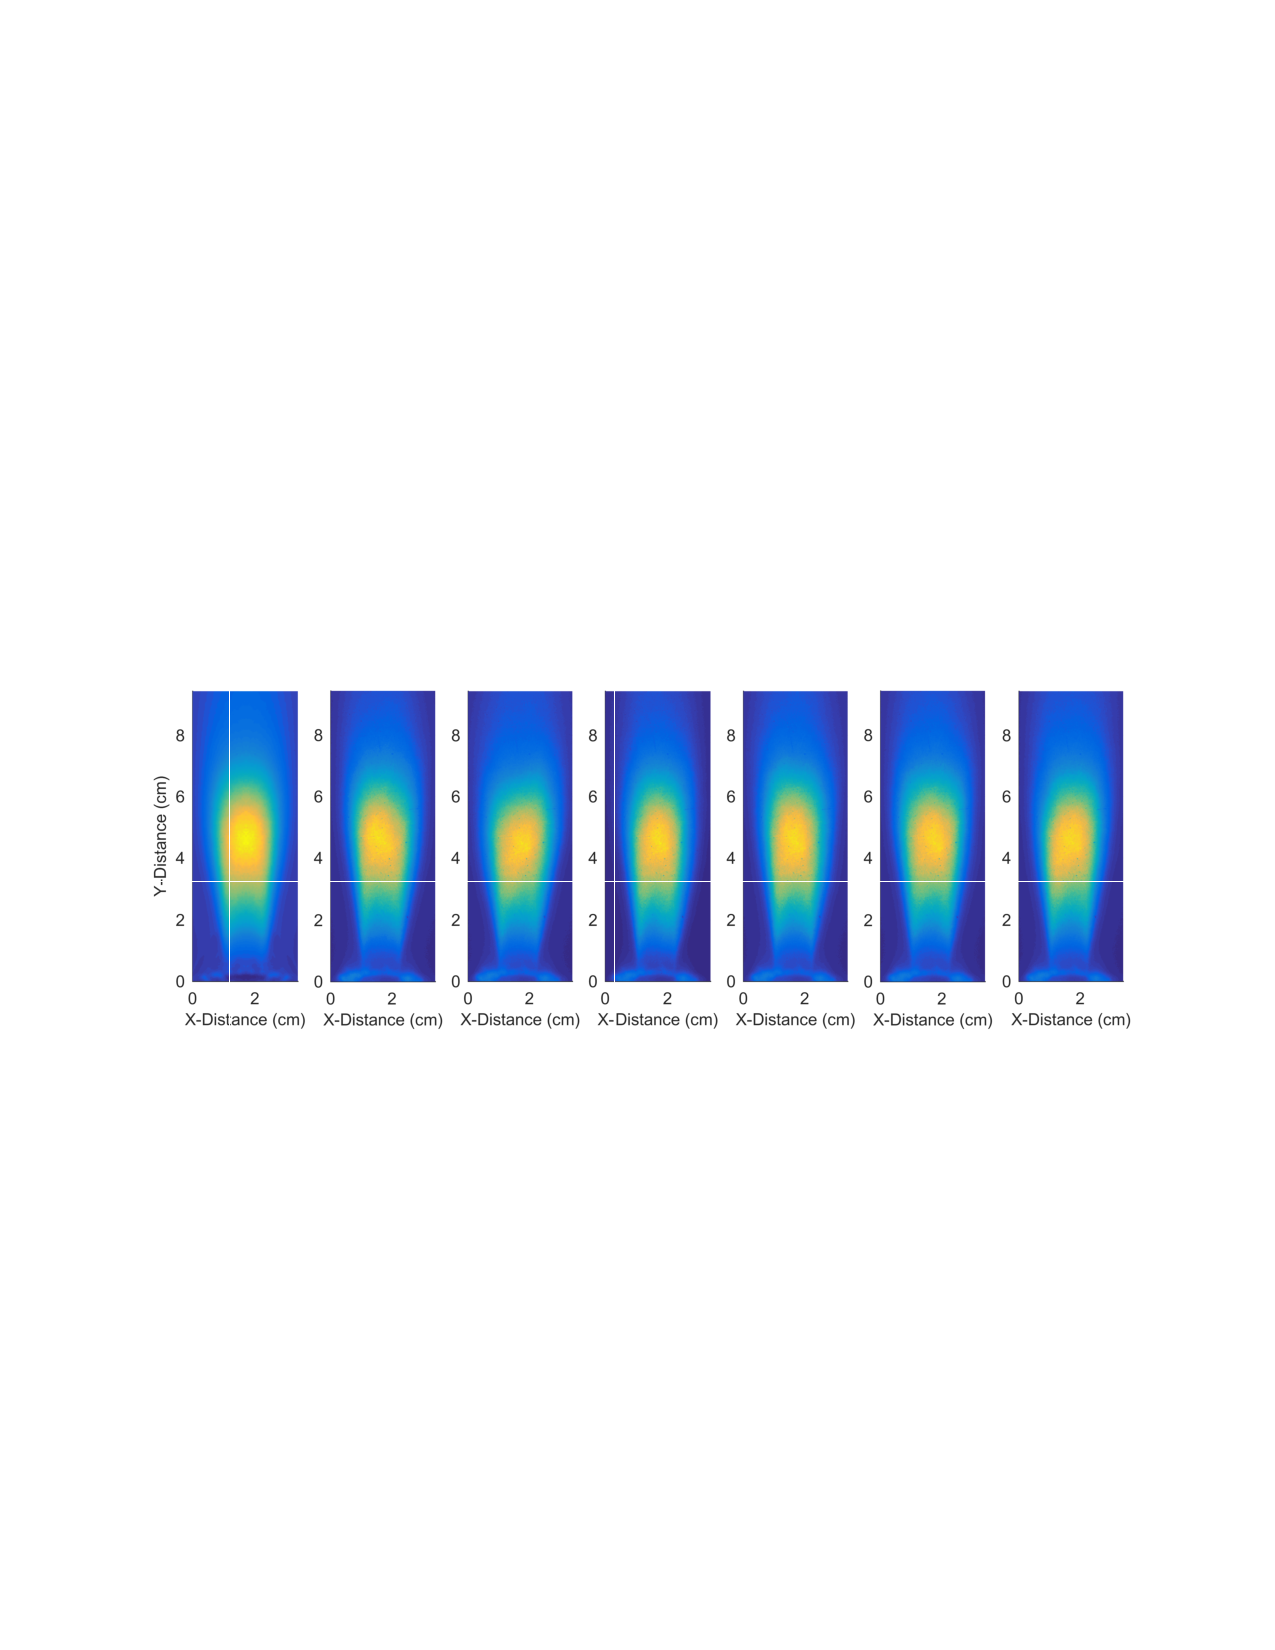
\includegraphics[width=.95\textwidth]{Re10kHigh.pdf}
\caption{Flame with a Reynolds number of 10,000 and high turbulence intensity.  The combined time-averaged flame is shown on the left, and the flame area was found to be approximately 6.81 $\textnormal{cm}^2$}
\label{fig:10high}
\end{figure}

\begin{figure}[ht]
\centering
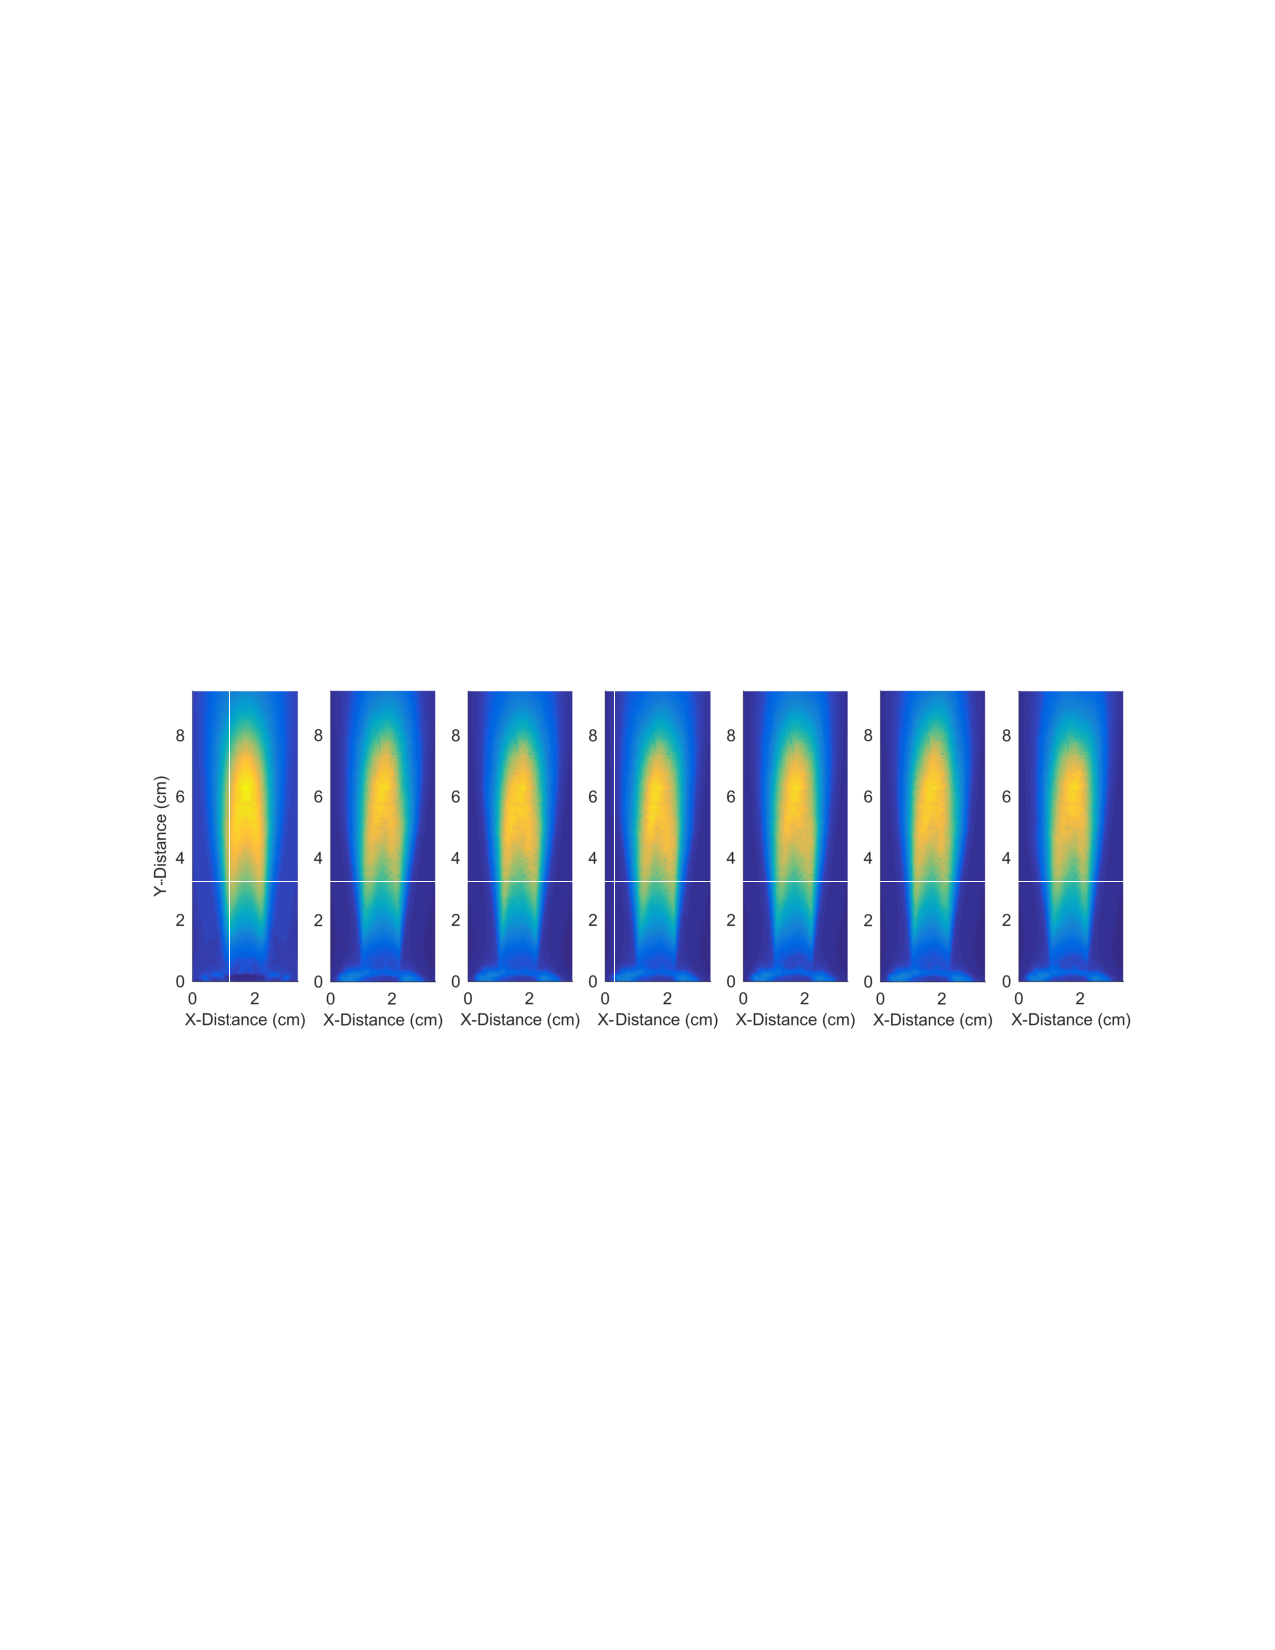
\includegraphics[width=.95\textwidth]{Re10kLow.pdf}
\caption{Flame with a Reynolds number of 10,000 and low turbulence intensity.  The combined time-averaged flame is shown on the left, and the flame area was found to be approximately 7.22 $\textnormal{cm}^2$}
\label{fig:10low}
\end{figure}

\clearpage


\section{Equipment and Tolerances}\label{app:Equip}

The same equipment used in previous flow calibration experiment was used in the burner apparatus.  Not all flow calibration equipment was used in the current experiment (i.e. the dry test meter and scale were not directly used for measurements of either the pilot or the turbulent flame), however for sake of completeness the equipment from the flow control experiment is included below:

\begin{table}[h]
	\begin{adjustwidth}{-1in}{-1in}
	\begin{center}
	\begin{tabular}{ | c  c  c |}
	 \hline
	 Instrument & Model & Tolerance \\
	 \hline\hline
	 Orifice & O'Keefe Type H & See Table \ref{tab:orif} \\
	 \hline
	 Rotameter & Omega FL4611-V & +/- 2.5\% of Full Scale (0.2125 scfm)\\
	 \hline
	 Pressure Transducer & Omega PX309 & +/- 0.25\% Full Scale (.25 psi) \\
	 \hline
	 Thermocouple & Type K & +/- \(2.2^\circ\)C \\
	 \hline
	 Dry Test Meter & Singer DTM-200\footnote{The American Meter division of Singer was acquired through a series of transactions by Elster American Meter, therefore 		specifications on the Elster American Meter DTM-200 are assumed to be identical to the Singer DTM-200.} & +/- 0.01 standard cubic foot \\
	 \hline
	 Pump & Isco-pump Series D & +/- 0.1\% \\
	 \hline
	 Scale & AND FX-6000 & +/- 0.1 gram \\
	 \hline
	 Bubble Calibrator & Gilian Gilibrator D800268 & +/- 1\% of reading accuracy \\
	 \hline
	 Thermal Flow Controller & MKS GM50A & +/- 1\% of set point \\
	 \hline
	\end{tabular}
	\caption{Equipment Used}\label{tab:tol}
	\end{center}
	\end{adjustwidth}
\end{table}

The orifice used in Laboratory 1 was placed in service in this experiment.  Its critical dimensions are as follows:

\begin{table}[h]
\begin{center}
\begin{tabular}{ | c  c  c |}
 \hline
 Measurement & Nominal Value & Tolerance \\
 \hline
 Orifice Diameter & 0.1248 inch & +/- 0.0004472 inch \\
 \hline
 Upstream Diameter & 0.3105 inch & +/- 0.0009617 inch \\
 \hline
\end{tabular}
\end{center}
\caption{Orifice Dimensions}\label{tab:orif}
\end{table}

In addition to the equipment used in Laboratory 1, an ICCD camera was used:

\begin{table}[h]
\begin{center}
\begin{tabular}{ | c  c  c |}
 \hline
 Manufacturer & Type & Model No. \\
 \hline
 Andor Technology Ltd. & iStar ICCD & DH334T-18U-E3 \\
 \hline
\end{tabular}
\end{center}
\caption{Camera Information}\label{tab:camera}
\end{table}




\clearpage


\section{MATLAB Code}\label{app:Code}

\begingroup
\fontsize{9pt}{12pt}\selectfont
\begin{verbatim}
clear
clc
close all
%% Add path to functions for calculating laminar and turbulent flame speeds.
% NOTE: if you bwfilter.m is not in the same directory that you run this in
% you will need to add a path for it.
Datapath = '/scratch';                           %Adds Data path as callable string
bg_path = {'RE_5000_Juan.tiff','RE_10000_Juan.tiff'};                         
%Background File Path
Cal_path = 'Spacial_Calibration_Group_Juan.tiff';                       
%Calibration File Path

numsamples = 1;                                                                 
%Number of sample's
numframes = 360*numsamples;                                                     
%Set number of frames from camera settings
home = pwd;                                                                    
%Sets variable "home" to current directory Callable

fg_path = {'A2_5k_HTI_01.tiff','A2_5k_HTI_02.tiff','A2_5k_HTI_03.tiff',...
    'A2_5k_LTI_01.tiff','A2_5k_LTI_02.tiff','A2_5k_LTI_03.tiff',...
    'A2_10k_HTI_01.tiff','A2_10k_HTI_02.tiff','A2_10k_HTI_03.tiff',...
    'A2_10k_LTI_01.tiff','A2_10k_LTI_02.tiff','A2_10k_LTI_03.tiff'};          
    %Forground File Path - This is your image of interest
%fg_path = 'C:\Users\cowand\ME 552 Data\A2_10k_LTI_03.tiff';
%fg_path = 'C:\Users\cowand\ME 552 Data\A2_10k_HTI_02.tiff';

%% Input Parameters
m_dot_total =0.001215;               %Total mass flow (kg/s) of reactants for Re=5,000
%m_dot_total=.00243;                 %Total mass flow (kg/s) of reactants for Re=10,000
rho_u       = 0.7871;                     %Unburned Density (kg/m^3) at 200 C
D           = 12/10;                       %Burner Diameter (cm)

%%  Spacial Calibration

%This will be used for image croping and spatial calibration
info_cal= imfinfo(Cal_path);

im_cal=imread(Cal_path,1,'Info',info_cal,'PixelRegion',{[775,921],[300,900]});
figure(15)
imshow(im_cal,[50,230]); axis image %This will show the image to calibrate to
title('Select locations 70cm and 76cm') %Please select locations 70cm and 76cm
points=ginput(2);
close
point_dist=pdist(points,'euclidean');
cal_val=6/point_dist; %Image calibration  (cm/pixel)

%% Image Cropping

center_l=514;                       %axis of symetry
Lcrop= 420;                       % left edge of the Burner
Rcrop= 1024+Lcrop-2*center_l;                       % right edge of the Burner
Tcrop= 400;                       % location for cropping of the top of the image
Bcrop= 1024-921;                       % location for cropping of the bottom of the image

%% Background images

for f=1:length(bg_path) %finding backgound info for both Re
    info_b=imfinfo(bg_path{f}); %info of image
    for i=1:numframes %calculating the background average
        if i==1
            im_avg_b=double(imread(bg_path{f},1,'Info',info_b,'PixelRegion',...
            {[Tcrop,1024-Bcrop],[Lcrop,1024-Rcrop]}));
        else
            image_i=double(imread(bg_path{f},i,'Info',info_b,'PixelRegion',...
            {[Tcrop,1024-Bcrop],[Lcrop,1024-Rcrop]}));
            im_avg_b=((i-1).*im_avg_b+image_i)./i;
        end
    end
    b_avg(:,:,f)=im_avg_b; %This has both Re values in it.
end

%% Building Meshgrid 

siz=size(im_avg_b); %Used to greate mesh grid
x=0:(siz(2)-1); 
x=cal_val*x; %Calibrated x distance
y=0:(siz(1)-1); 
y=cal_val*y; %Calibrated y distance
y=fliplr(y);

[X,Y]=meshgrid(x,y);
%Y=flipud(Y);

%% Calculating averages and plotting images


count=1;
for f=1:length(fg_path) %Plotting all files
    info_f=imfinfo(fg_path{f}); %info of image


    for i=1:numframes %calculating the image average
        if i==1
            image_0=double(imread(fg_path{f},1,'Info',info_f,'PixelRegion',...
            {[Tcrop,1024-Bcrop],[Lcrop,1024-Rcrop]}));
            im_avg_f=image_0;
        else
            image_i=double(imread(fg_path{f},i,'Info',info_f,'PixelRegion',...
            {[Tcrop,1024-Bcrop],[Lcrop,1024-Rcrop]}));
            im_avg_f=((i-1).*im_avg_f+image_i)./i;
        end
    end
    
    f_avg(:,:,f)=im_avg_f; %Image average per test. This has both Re values in it.
    
    if f<6.5 %The following is calculating the flame minus the background
        flame_avg(:,:,f)=f_avg(:,:,f)-b_avg(:,:,1);
    else
        flame_avg(:,:,f)=f_avg(:,:,f)-b_avg(:,:,2);
    end
    
%    max_int=max(max(flame_avg(:,:,f))); %finding maxinum intensity for per test
    flame_avg(:,:,f)=medfilt2(flame_avg(:,:,f)); %filters
    flame(:,:,f)=0.5*(flame_avg(:,1:end,f) + flame_avg(:, end+1-(1:end), f));   
    % Axis symetric

    
    if rem(f,3)==0 %This is to find the average with all three tests
        avg_flame(:,:,count)=mean(flame(:,:,f-2:f),3);
        if f<3.5 %Plotting average to compare to snap-shots
            figure(1)
            subplot(1,7,1)
            surf(X,Y,avg_flame(:,:,count),'EdgeColor','None'); axis image
            view(2)
            xlim([0,max(x)])
            ylim([0,max(y)])
            xlabel('X-Distance (cm)')
            ylabel('Y-Distance (cm)')
        elseif f<6.5
            figure(2)
                        
            subplot(1,7,1)
            surf(X,Y,avg_flame(:,:,count),'EdgeColor','None'); axis image
            view(2)
            grid off
            xlim([0,max(x)])
            ylim([0,max(y)])
            xlabel('X-Distance (cm)')
            ylabel('Y-Distance (cm)')
        elseif f<9.5
            figure(3)
                
            subplot(1,7,1)
            surf(X,Y,avg_flame(:,:,count),'EdgeColor','None'); axis image
            view(2)
            grid off
            xlim([0,max(x)])
            ylim([0,max(y)])
            xlabel('X-Distance (cm)')
            ylabel('Y-Distance (cm)')
        else
            figure(4)
                       
            subplot(1,7,1)
            surf(X,Y,avg_flame(:,:,count),'EdgeColor','None'); axis image
            view(2)
            grid off
            xlim([0,max(x)])
            ylim([0,max(y)])
            xlabel('X-Distance (cm)')
            ylabel('Y-Distance (cm)')
        end
        count=count+1;
    end
    
    title_loc=4; %Location of center of title over which sub plot
    
    if f<3.5 %The following if statement plots the 6 snap-shots
        figure(1)
        a=f;
        subplot(1,7,a+1)
        surf(X,Y,image_0,'EdgeColor','None'); axis image %one snap shot per test
        view(2)
        xlim([0,max(x)])
        ylim([0,max(y)])
        xlabel('X-Distance (cm)')
        %ylabel('Y-Distance (cm)')
        
        subplot(1,7,a+4)
        surf(X,Y,image_i,'EdgeColor','None'); axis image %The other snap shot per test
        view(2)
        xlim([0,max(x)])
        ylim([0,max(y)])
        xlabel('X-Distance (cm)')
        %ylabel('Y-Distance (cm)')
    
    elseif f<6.5
        figure(2)
        
        a=f-3;
        subplot(1,7,a+1)
        surf(X,Y,image_0,'EdgeColor','None'); axis image %one snap shot per test
        view(2)
        xlim([0,max(x)])
        ylim([0,max(y)])
        xlabel('X-Distance (cm)')
        %ylabel('Y-Distance (cm)')
        
        subplot(1,7,a+4)
        surf(X,Y,image_i,'EdgeColor','None'); axis image %The other snap shot per test
        view(2)
        xlim([0,max(x)])
        ylim([0,max(y)])
        xlabel('X-Distance (cm)')
        %ylabel('Y-Distance (cm)')

    elseif f<9.5
        figure(3)

        a=f-6;
        subplot(1,7,a+1)
        surf(X,Y,image_0,'EdgeColor','None'); axis image %one snap shot per test
        view(2)
        xlim([0,max(x)])
        ylim([0,max(y)])

        xlabel('X-Distance (cm)')
        %ylabel('Y-Distance (cm)')
        
        subplot(1,7,a+4)
        surf(X,Y,image_i,'EdgeColor','None'); axis image %The other snap shot per test
        view(2)
        xlim([0,max(x)])
        ylim([0,max(y)])
        xlabel('X-Distance (cm)')
        %ylabel('Y-Distance (cm)')

    else
        figure(4)
       
        a=f-9;
        subplot(1,7,a+1)
        surf(X,Y,image_0,'EdgeColor','None'); axis image %one snap shot per test
        view(2)
        xlim([0,max(x)])
        ylim([0,max(y)])

        xlabel('X-Distance (cm)')
        %ylabel('Y-Distance (cm)')
        
        subplot(1,7,a+4)
        surf(X,Y,image_i,'EdgeColor','None'); axis image %The other snap shot per test
        view(2)
        xlim([0,max(x)])
        ylim([0,max(y)])
        xlabel('X-Distance (cm)')
        %ylabel('Y-Distance (cm)')

    end
    
end

figure(1)
suptitle('Axis Symetric Corrected Flame (Re=5,000, High Turbulence Intensity)')

figure(2)
suptitle('Axis Symetric Corrected Flame (Re=5,000, Low Turbulence Intensity)')

figure(3)
suptitle('Axis Symetric Corrected Flame (Re=10,000, High Turbulence Intensity)')

figure(4)
suptitle('Axis Symetric Corrected Flame (Re=10,000, Low Turbulence Intensity)')


%% Finding flame area
center=(siz(2)+1)/2; %center index
%figure(11)
%plot(y,movmean(avg_flame(:,center,2),20))
%plot(h,max1h)


for i=1:4
    flamepixels(i) = 0;
    xpixelcount = length(avg_flame(:,1,i));
    ypixelcount = length(avg_flame(1,:,i));
    for j = 1:xpixelcount
        for k = 1:ypixelcount
            if avg_flame(j,k,i) > 24
                flamepixels(i) = flamepixels(i) + 1;
            end
        end
    end
    flame_A(i) = flamepixels(i) * cal_val^2;
end

flame_A

end
\end{verbatim}
\endgroup


\end{appendices}
\end{document}